
In this chapter, the table space organization for both variant and subsumption tabling engines are described.
First, the variant table space for both SLG-WAM and YapTab is explained. Because
they share a lot of similarities, the description covers the common ground between the two systems.
Next, we explore two known mechanisms that
modify the previous table space for call by subsumption. Those two mechanisms have already been implemented in XSB
\cite{Rao-96, Johnson-99}.

\section{Table Space} \label{sec:table_space}

Implementing a tabling engine on a Prolog system involves the design of compact and time efficient data structures
to organize the table space. The table space is heavily used throughout the evaluation process in various operations:

\begin{itemize}
  \item to lookup if a subgoal is in the table, and if not insert it;
  \item to verify wether a newly found answer is already in the table, and if not insert it;
  \item to retrieve answers for consumer nodes.
\end{itemize}

\subsection{Tries}

Clearly, the success of tabling is highly dependent on the data structures used.
Both Yap \cite{Rocha-00a} and XSB \cite{RamakrishnanIV-95} use a trie-based tabling approach.

Tries were initially proposed to index dictionaries \cite{Fredkin-62} and have since been generalized to index recursive data structures
such as terms. The essential idea underlying a trie is to partition a set $T$ of terms based upon their structure,
hence common term prefixes are represented only once.

A trie is a tree-structured automaton with the root as the start state and each leaf state is associated with a term in $T$.
Each state specifies the position to be inspected in the input term on reaching that state.
The outgoing transitions specify the function symbols expected at that position.
A transition is taken if the current symbol in the input term matches the symbol of the transition.
If we recursively reach a leaf state we say that the input term \textit{matches} the term represented by the leaf state.
A complete path, from the root to a leaf, corresponds to a pre-order traversal of the matching term.
If no transition can be taken, the lookup operation fails. On the other hand, for an insert operation
we add a new outgoing transition for the current input symbol and a new node, which is linked to this transition.
To complete the insert operation, we consume the rest of the input term, until a leaf node is created that represents
the newly inserted term.

Given the nature of tries, the following conclusions can be made:

\begin{itemize}
  \item it is possible to do a single pass check/insert. If the lookup
  fails, it is possible to complete an insert operation using the last lookup state;
  \item the efficiency and memory consumption of a
  particular trie depends on the percentage of terms that have common prefixes.
\end{itemize}

When creating transitions for variables, we use the format outlined by Bachmair \textit{et al} \cite{Bachmair-93},
described in Section \ref{sec:variant_tabling}.

\begin{figure}[ht]
  \centering
    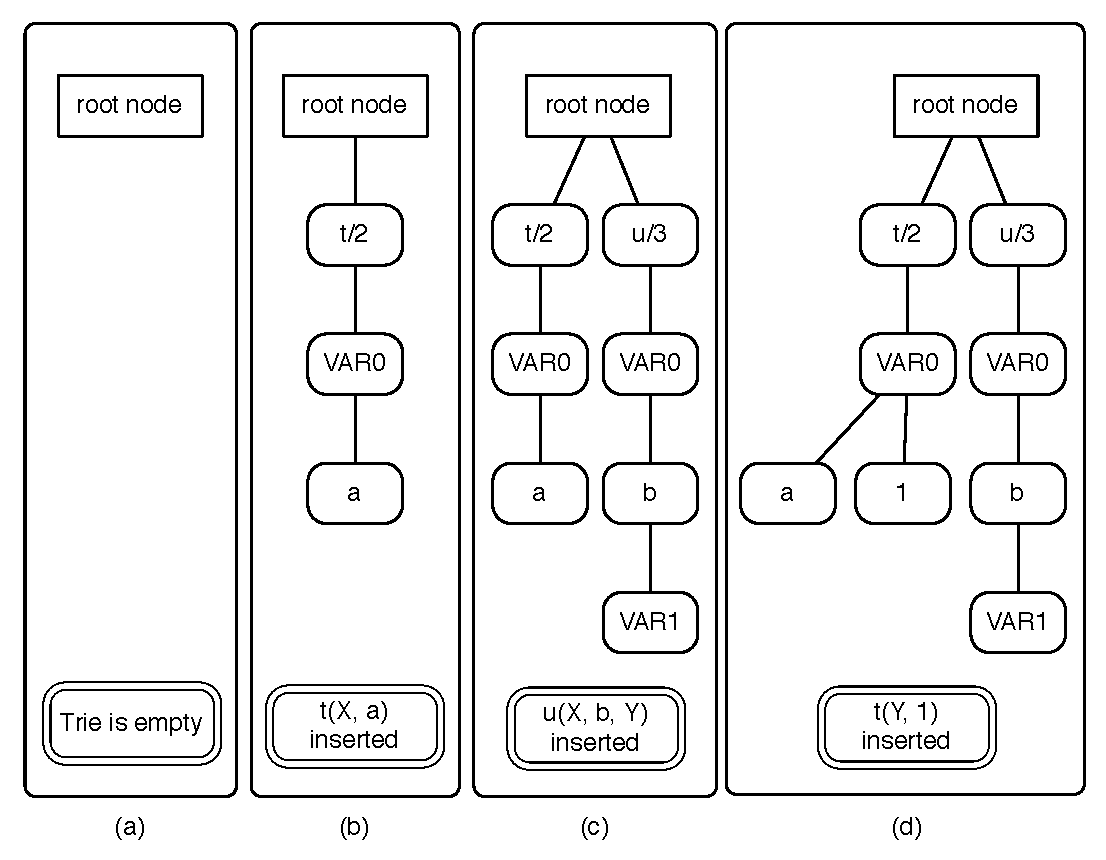
\includegraphics[scale=0.6]{tries.pdf}
  \caption{Using tries to represent terms.}
  \label{fig:tries_use}
\end{figure}

Figure \ref{fig:tries_use} shows a trie with three terms. First, in \textbf{(a)} the trie is represented by a \textit{root node} and has
no terms. Next, in \textbf{(b)} the term \texttt{t(X,a)} is inserted and three nodes are created that represent each part of the term.
In \textbf{(c)} a new term, \texttt{u(X,b,Y)} is inserted. This new term differs from the first one and a new distinct branch is created.
Finally, in \textbf{(d)}, the input term is \texttt{t(Y,1)} and only a new node needs to be created as this term shares two nodes
with \texttt{t(X,a)}.

Yap and XSB use two levels of tries to implement tabling:

\begin{itemize}
  \item One level stores subgoal calls for each predicate;
  \item The second level stores answers for a specific subgoal.
\end{itemize}

\begin{figure}[ht]
   \centering
     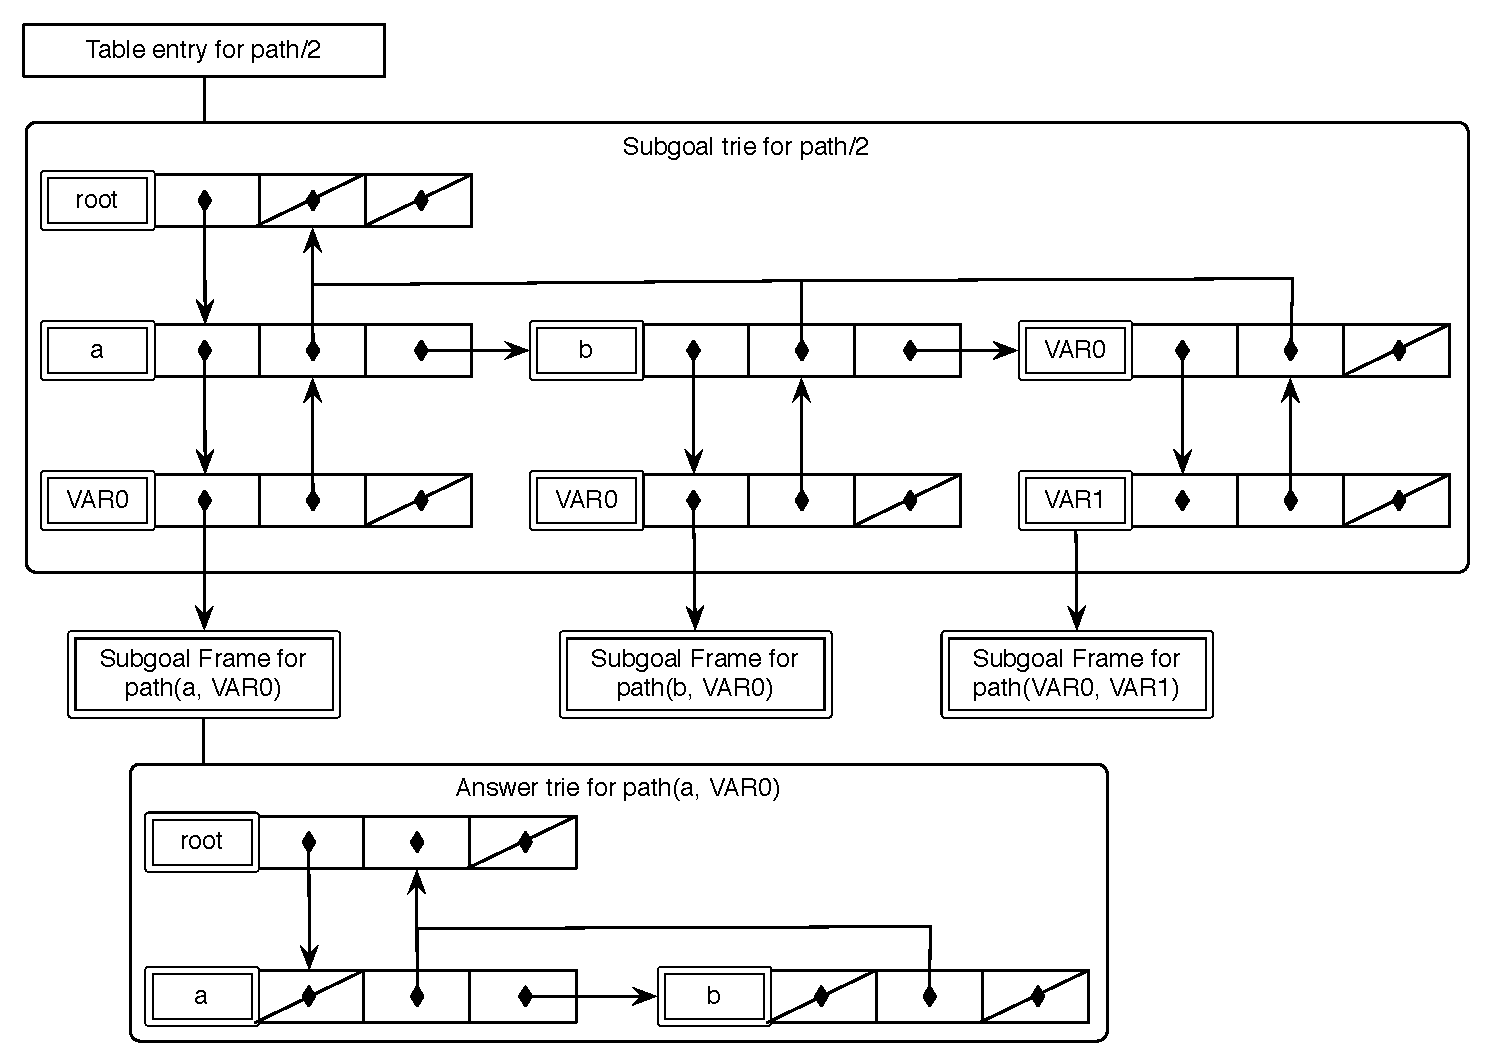
\includegraphics[scale=0.6]{two_level_tries.pdf}
   \caption{Organizing the table space with tries for variant tabling.}
   \label{fig:table_space_tries}
 \end{figure}

For both levels, each trie node usually contains four fields. The first field represents the \textbf{symbol} (or \textbf{atom})
of the transition. The second points to the first descendant transition (called the \textbf{child node})
and the third stores a pointer to the \textbf{parent} node.
The fourth field points to a \textbf{sibling} node.

When the chain of sibling nodes gets too big, an hashing scheme is dynamically employed to provide direct
access to nodes, optimizing the search of transitions.

Each tabled predicate contains a \textit{table entry} that points to a \textit{subgoal trie}.
Only the subgoal arguments are stored.
Each different call to a tabled predicate corresponds to a unique path through the trie.
The leaf points to a data structure called \textit{subgoal frame}. The frame stores
information about the subgoal, namely an entry point to its \textit{answer trie}.

The answer trie stores answers to the subgoal. When inserting answers only substitutions
for the variables in the call are stored. This optimization is called \textit{substitution factoring} \cite{RamakrishnanIV-95}.

Figure \ref{fig:table_space_tries} shows the table space after evaluating \texttt{path(X,Z)} (example in Figure \ref{fig:tabling_path}).
Subgoals \texttt{path(X,Z)}, \texttt{path(b,Z)} and \texttt{path(a,Z)} are stored in the \texttt{path/2} subgoal trie.
Only the answer trie for \texttt{path(a,Z)} is represented. Using substitution factoring only \texttt{Z = b} and \texttt{Z = a}
are stored.

\subsection{Subgoal Frames}

A subgoal frame contains general information about the state of a tabled subgoal.
To access answers, this frames contain a pointer to the root of the answer trie.

A chain of answers used by consumers is also kept in the form of head and tail pointers.
In XSB, a \textit{answer return list} is built and the consumer has a pointer to the last consumed node of the list.
In Yap, answers are chained using the \textbf{child} pointer of the leaf answer nodes. Yap's consumers only keep
the last consumed answer leaf. The last consumed answer pointer is an \textit{answer continuation}. Thus, when
a consumer needs to verify or consume the next available answer, it uses the continuation to retrieve the next
answer, following the chain of answers. To load an answer, the trie nodes are traversed in bottom-up order and the answer is reconstructed.

To facilitate memory management, both systems link subgoal frames by storing \textbf{next} and \textbf{previous} pointers in each subgoal frame,
forming a double linked list.

Information about the current evaluation state of the subgoal is usually kept. Yap has the following states:
\textit{ready}, \textit{evaluating}, \textit{complete} and \textit{incomplete}.

\section{Tabling by Call Subsumption} \label{sec:subsumption}

Although variant based tabling has proven to be greatly beneficial in solving some shortcomings of the SLD resolution,
other approaches are possible. Tabling by call subsumption aims to reuse answer computations by sharing answers from
\textit{more general} goals \cite{Johnson-99}.

When a subgoal is first called, a variant engine will lookup in the table space for a variant subgoal, one that is
identical by renaming the variables. If a subgoal already exists on the subgoal trie, a new consumer is created which
consumes answers from the variant subgoal.

Although a variant check is a light-weight operation computationally,
tabling engines using such checks can end up computing answers through program clause resolution, which takes time and space,
when they could retrieve answers from a subgoal that \textit{subsumes} the new call. By other words, a more specific subgoal
could consume answers from a general subgoal, which contains the full set of answers for the specific subgoal among the complete set.

Formally, if two subgoals $G$ and $G'$ exist, such that $S$ and $S'$ are the respective answer sets and
$G'$ subsumes $G$, we can conclude that $S \subseteq S'$.

The effects of using subsumptive checks are greater reuse of computed answers and reduced program clause resolution, yielding
superior time performance. In terms of space, improvements can be made since fewer calls and their associated answer sets
need to be preserved \cite{Johnson-99}.
However, implementing call subsumption poses various challenges:

\begin{enumerate}[(a)]
\item How to efficiently check for subsuming subgoals in the subgoal trie;
\item How to design new mechanisms to represent answers supporting fast retrieval of subsets that are only related to a subsumed call;
\item How to support incremental retrieving of the answer subset. Note that, during evaluation, it may be not possible for
the subsuming call to contain all answers, as the process of generating answers is incremental.
\end{enumerate}

For illustration purposes, in Figure \ref{fig:tabling_path_sub}, we describe the evaluation of \texttt{path(X,Z)}
using the program presented in Figure \ref{fig:prolog_path}
and compare it against the variant approach in Figure \ref{fig:tabling_path}.

\begin{figure}[ht]
\centering
  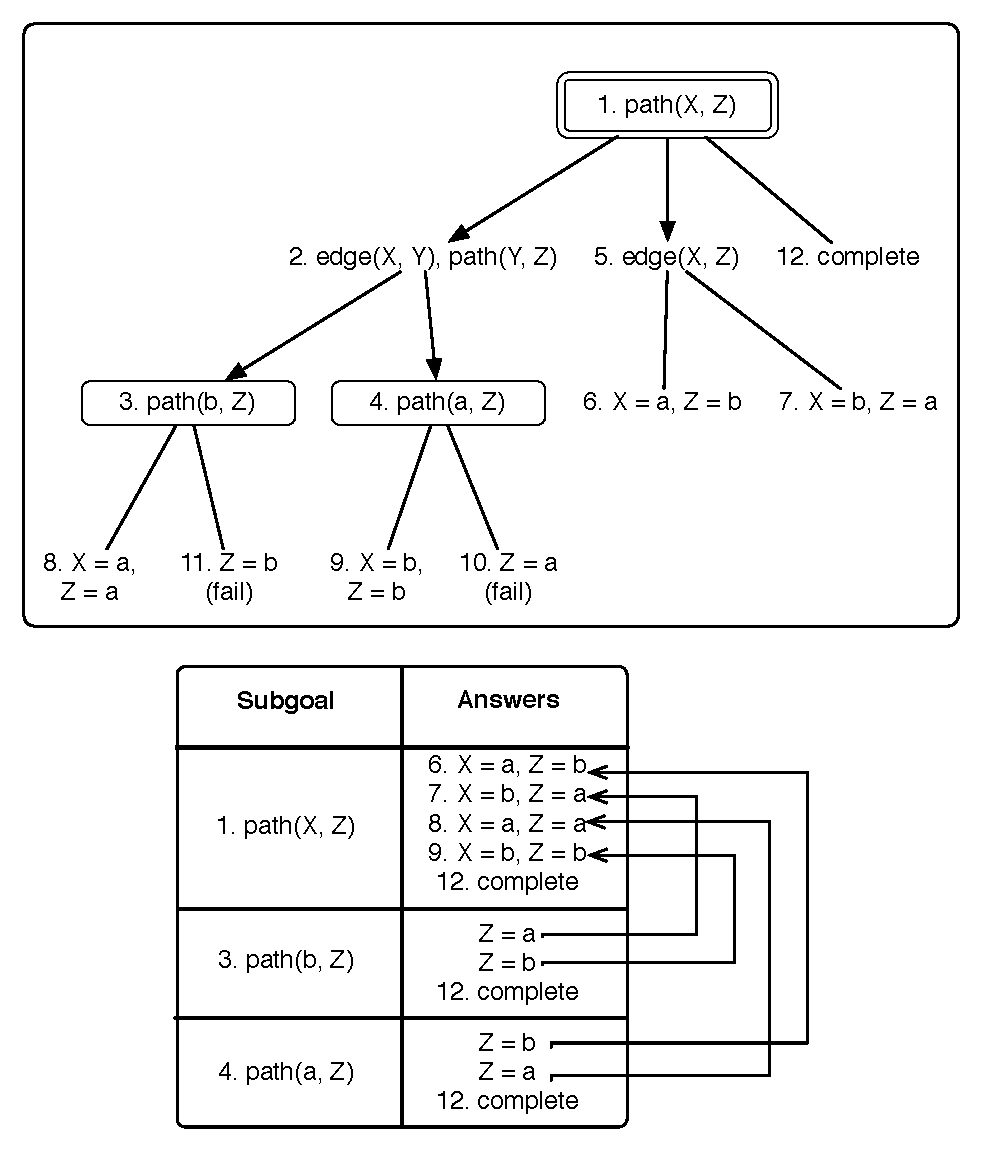
\includegraphics[scale=0.6]{tabling_path_sub.pdf}
\caption{Tabling \texttt{path(X,Z)} using call by subsumption.}
\label{fig:tabling_path_sub}
\end{figure}

At step 1 the subgoal \texttt{path(X,Z)} is called and a new generator node is created as there is no existing subgoals in the table space
that could be variant or subsuming. Being a generator node, it is evaluated using the program clauses (step 2). The first solution
for the \texttt{edge(X,Y)} predicate is evaluated using Prolog's standard rules and yields a subgoal call to \texttt{path(b,Z)} (step 3).

In variant tabling the engine would search for a variant subgoal in the table space, thus failing and creating a new generator node,
meanwhile expanding the execution tree by means of program clause resolution. In subsumptive tabling, the engine searches for a subsuming call,
and finds \texttt{path(X,Z)}. This subgoal
is more general than \texttt{path(b,Z)} and contains all the answers need for the subsumed goal.
A special type of consumer called a \textit{subsumptive consumer} is created. This consumer knows the subsuming subgoal and can retrieve
the answers that unify with the subsumed call.

As \texttt{path(X,Z)} has no answers and thus, no answers that can be consumed by \texttt{path(b,Z)}, the consumer node is suspended
and execution backtracks to node 2. The second clause of \texttt{edge/2} is tried and a new tabled subgoal is called: \texttt{path(a,Z)} (step 4).
Like \texttt{path(b,Z)}, this subgoal is subsumed by \texttt{path(X,Z)}, hence a new subsumptive consumer node is created. Execution suspends
once again because no answers are available and the engine goes back to node 1 to try the second \texttt{path/2} clause (step 5).

Solutions for \texttt{path(X,Z)} are found in steps 6, \texttt{X = a, Z = b}, and 7, \texttt{X = b, Z = a}. They are stored in the answer set
for this generator node. Execution thus backtracks to node 1 and completion is attempted. Node 1 verifies that node 3 and 4 have
unconsumed answers and starts by resuming computation at node 3.

Node 3 being a subsumptive consumer looks up in the \texttt{path(X,Z)}
answer set for answers specific to \texttt{path(b,Z)}, finding one: \texttt{Z = a}. At this point, the consumer marks the answer
for later retrieval, so that answers can be immediately consumed when a variant subgoal is called.
Like variant tabling, the consumer keeps a last consumed answer continuation to know which answers have already been consumed.
Variable bindings for this answer are propagated and a new answer to \texttt{path(X,Z)} is found: \texttt{X = a, Z = a} (step 8).
Node 3 tries to consume a new answer, but no new answers are available for this subgoal.

Execution suspends node 3 and resumes computation at node 4. Here \texttt{path(a,Z)} begins to consume answers from \texttt{path(X,Z)}
using the subsumption mechanism. The first answer in \texttt{path(X,Z)}, \texttt{X = a, Z = b}, unifies with the subsumed goal and
is consumed. By variable propagation, a new answer for \texttt{path(X,Z)} is also generated, \texttt{X = b, Z = b} (step 9).
Node 3 then tries to consume a new answer and finds \texttt{X = a, Z = a}. This new answer
is added to the \texttt{path(a,Z)} table space. As the new variable bindings are propagated, a new answer is also generated
for top subgoal, but the answer is repeated (\texttt{X = b, Z = a}) (step 10), and hence it is not inserted into the table space.

As each consumer uses the available answers, execution backtracks to the leader node, \texttt{path(X,Z)}, that will once
again attempt completion. By using the last consumed answer continuation, it verifies that node 3 has unconsumed answers.
Execution thus resumes at node 3.

Node 3 inspects \texttt{path(X,Z)} answer set and consumes the next matching answer, \texttt{X = b, Z = b}. A new answer
for \texttt{path(b,Z)} is generated and variable bindings are propagated to the leader node (step 11). The new answer is already
stored in the table space and it is not used.

Once again, evaluation returns to the leader node and completion is performed (step 12) as each consumer has exhausted the
available answers.

This evaluation example, when compared to variant tabling, shows a smaller execution tree with less
program clauses expanded. The subsumptive computation also took less steps to complete and a greater
reuse of answers was done between \texttt{path(X,Z)}, \texttt{path(b,Z)} and \texttt{path(a,Z)}.

Although this example shows a very good performance of this method of evaluation, if we tried
to evaluate \texttt{path(a,Z)} and then \texttt{path(X,Z)}, no reuse could be done with \texttt{path(a,Z)}
because no previous subsuming goal was present. The more general subgoals are called first, the greater
the reuse in call subsumption.

Like variant tabling, the same four main operations are used when evaluating subsumptive subgoals.
These operations are very similar, with a few differences. Operations \textit{new answer} and
\textit{completion} remain the same, while the \textit{tabled subgoal call} and \textit{answer resolution}
work differently:

\begin{itemize}
\item The \textit{tabled subgoal call} operation represents a call to a tabled subgoal.
If the subgoal $C$ is called, a search for a subsuming subgoal $C'$ is done. If such subgoal is found,
the new subgoal will be resolved using \textit{answer clause resolution}, thus consuming answers from the subgoal $C'$.
If no subgoal $C'$ is found, then $C$ is inserted into the table space and the new generator node is evaluated using
program clause resolution.

\item The \textit{answer resolution} operation checks wether new answers from the table space are available for consumption.
Each subsumptive consumer node uses an answer continuation that represents
the set of remaining answers to be consumed. Given an answer continuation we inspect the answer trie from the subsuming subgoal
and retrieve the next answer that matches with the subsumed goal. Once the answer is retrieved and loaded, the answer
continuation is updated to reflect the new answer consumed.
\end{itemize}

We next describe two known techniques that implement subsumptive tabling. These two approaches were both implemented in XSB.

\subsection{Dynamic Threaded Sequential Automata}\label{sec:dtsa}

\textit{Dynamic Threaded Sequential Automata} (DTSA) is a data structure that provides good indexing and incremental
returning of a subset of answers from a subsuming call to a subsumed call \cite{Rao-96}.

This structure orders answers as they are generated, hence it can easily mark which answers were already retrieved, enabling
efficient retrieval of the remaining answers.

A DTSA is based on a \textit{Sequential Factoring Automaton} (SFA) \cite{Dawnson-95} but has a few more features for dealing with fast indexing
and incremental retrieving of answers.

\subsubsection{Sequential Factoring Automaton}

A SFA solves the problem of retrieving an ordered subset of answers, starting from the oldest to the newest answer. It is an ordered
tree-structure automaton and is very similar to a trie. It starts with a root as the start state and has edges as transitions
that represent unifications. Every leaf represents a distinct term and the transitions on the path from the root to a leaf
represent the operations necessary to unify the goal with the term at the leaf.

Apart from ordering, SFAs differ from tries in that transitions from a state may not be unique and each transition in a trie
denotes match operations, not unify operations.

\begin{figure}[ht]
  \centering
    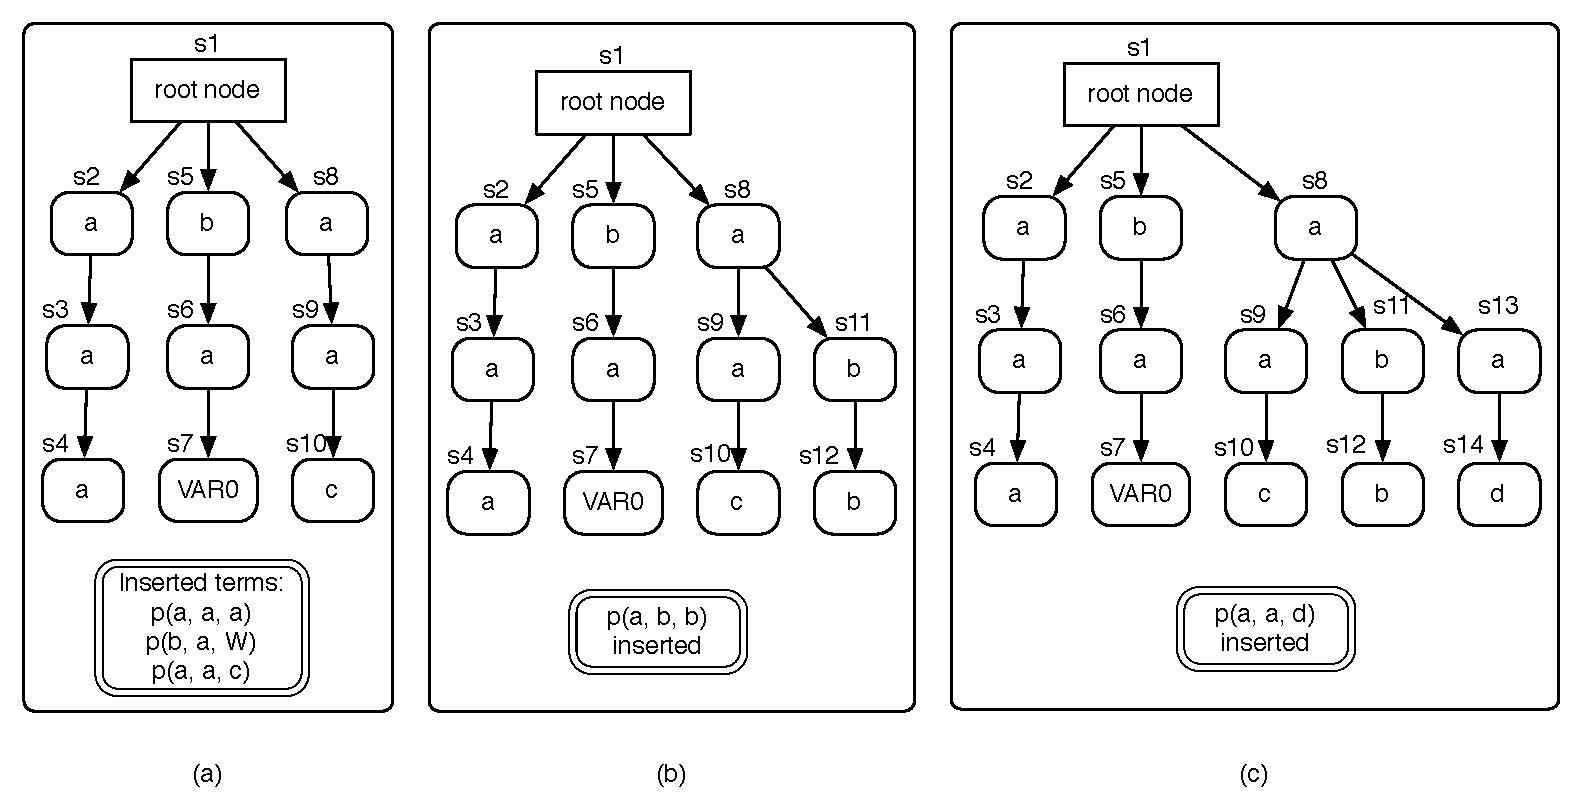
\includegraphics[scale=0.6]{sfa.pdf}
  \caption{Inserting answer terms in a SFA.}
  \label{fig:sfa_example}
\end{figure}

To insert a new term into a SFA, we must start by inserting symbols from the answer term into the root state.
In each state we verify if the last transition $s$ matches the current term symbol $t$. If $t$ matches $s$
we take the transition and advance to the next state; if not, a new transition for $t$ is created and we advance
to the newly created state. When all term symbols $t$ are exhausted, the current state is marked as a leaf,
representing a new answer.
Figure \ref{fig:sfa_example} represents a SFA for the subgoal \texttt{p(X,Y,Z)} and
illustrates insert operations.

When a new subgoal $G$ subsumed by the subgoal $G'$ is first called, we must determine the assignments
from $G'$ to the sub-terms of $G$, because only variable substitutions are inserted into a SFA.
The assignments are usually stored under the choice point.

For example, if $G'$ is \texttt{p(X,Y,Z)} and $G$ is \texttt{p(a,a,V)}, the variable assignments
are \texttt{X = a, Y = a, Z = VAR0}. During unification operations, we must unify the first SFA symbol
to $a$, then to $a$ again, and finally with \texttt{VAR0}.
Once a variable is \textit{bound}, subsequent unify operations must unify with the bounded sub-term.

The unification process starts in the root state with an empty \textit{continuation stack}.
When a state $s$ is reached, the leftmost transition that unifies with the current $G$ assignment is chosen,
this is called the \textit{applicable transition}.
Before moving to the next state, we select the next applicable transition and push it on the continuation stack.
If no applicable transitions are available at state $s$ or if an answer was found, we pop a transition from
the stack and use it to search for more answers. Once no more transitions can be taken and the stack is empty, the
search process ends.

Using the SFA in Figure \ref{fig:sfa_example} and the subgoal $G$, \texttt{p(a,a,V)}, the search mechanism starts
at the root state and is ready to retrieve all answers that unify with $G$.
The first applicable transition is $s1 \rightarrow s2$ because it unifies with the first symbol: $a$. The transition
$s1 \rightarrow s5$ can not be pushed into the continuation stack because it does not unify, but $s1 \rightarrow s8$ does.
In state $s2$ only one transition is available, thus nothing is pushed into the stack.
Transition $s2 \rightarrow s3$ unifies with symbol $a$ and we move to state $s3$. Here, the variable \texttt{VAR0} (that represents \texttt{V})
can unify with $a$, thus we can get to state $s4$, arriving at a leaf state and a new answer, \texttt{V = a}.

Next, the process must use the continuation stack to retrieve more answers. Transition $s1 \rightarrow s8$ is popped from the stack
and we arrive at state $s8$ with 3 available transitions. Using the previous rules, a new answer is retrieved,
\texttt{V = c} and the continuation stack contains the transition $s8 \rightarrow s13$.

Finally, once states $s8$, $s13$ and $s14$ are visited, the process arrives at a leaf state and a new answer, \texttt{V = d}, is retrieved.
The process finishes and every answer that is specific to \texttt{p(a,a,V)} is found.

\subsubsection{Threaded Sequential Automata}

A \textit{Threaded Sequential Automata} extends the SFA with a concept called
\textit{equivalent states}. One state $S1$ is equivalent to state $S2$ if when $S1$ is taken, $S2$ is also
guaranteed to be visited. For example, in Figure \ref{fig:sfa_example}, whenever states $S2$ and $S8$ are
visited, states $S8$ and $S9$ are also guaranteed to be visited, as they denote the same path.

A SFA is converted to a TSA by adding \textit{equivalence links} between equivalent states.
The SFA in Figure \ref{fig:sfa_example} was transformed into a TSA in Figure \ref{fig:tsa_example}.

\begin{figure}[ht]
  \centering
    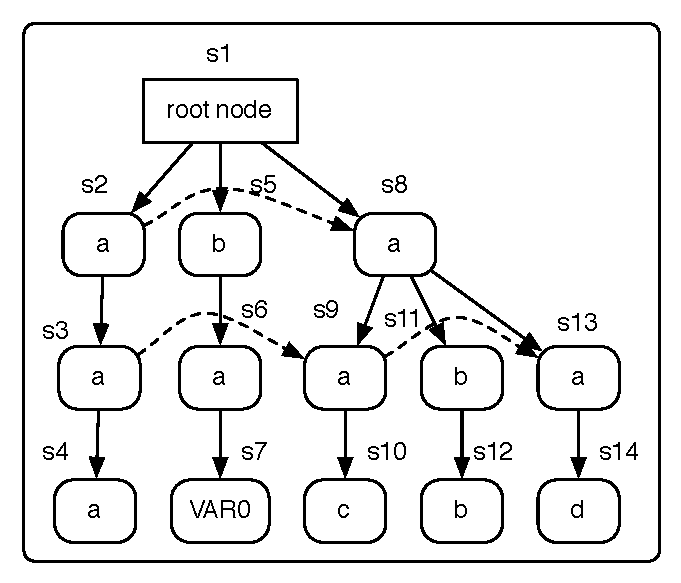
\includegraphics[scale=0.6]{tsa.pdf}
  \caption{SFA transformed into a TSA.}
  \label{fig:tsa_example}
\end{figure}

In the TSA, the concept of applicable transitions is changed. Now it is also possible to push equivalence links
into the continuation stack as if they were normal transitions. So, if we were at state $s3$ we use
the transition to $s9$ and then to $s13$ instead of going from the start state.

Although equivalence links provide an efficient indexing mechanism, they must be used with care. If not,
some situations arise where following equivalence links lead to repeated answers and answers in the incorrect order \cite{Rao-96}.
The selection of transitions must consider only \textit{safe transitions}, which reach answers that cannot be reached through the pending
transitions on the stack.
So, if the process is at state $s2$ and the transition $s1$ to $s8$ is already on the
stack, we can not use the equivalence link $s2 \rightarrow s8$, as the transition $s1$ to $s8$ already covers the same branch.

If we followed only safe transitions, no equivalence links would be used, hence we must check if there is any
equivalence link that can be used in the next state that covers the same answers if we pushed the
usual next applicable transition into the stack. Thus, at state $s2$ we would use the equivalence $s2$ to $s8$, instead of
the transition $s1 \rightarrow s8$.

\begin{figure}[ht]
  \centering
    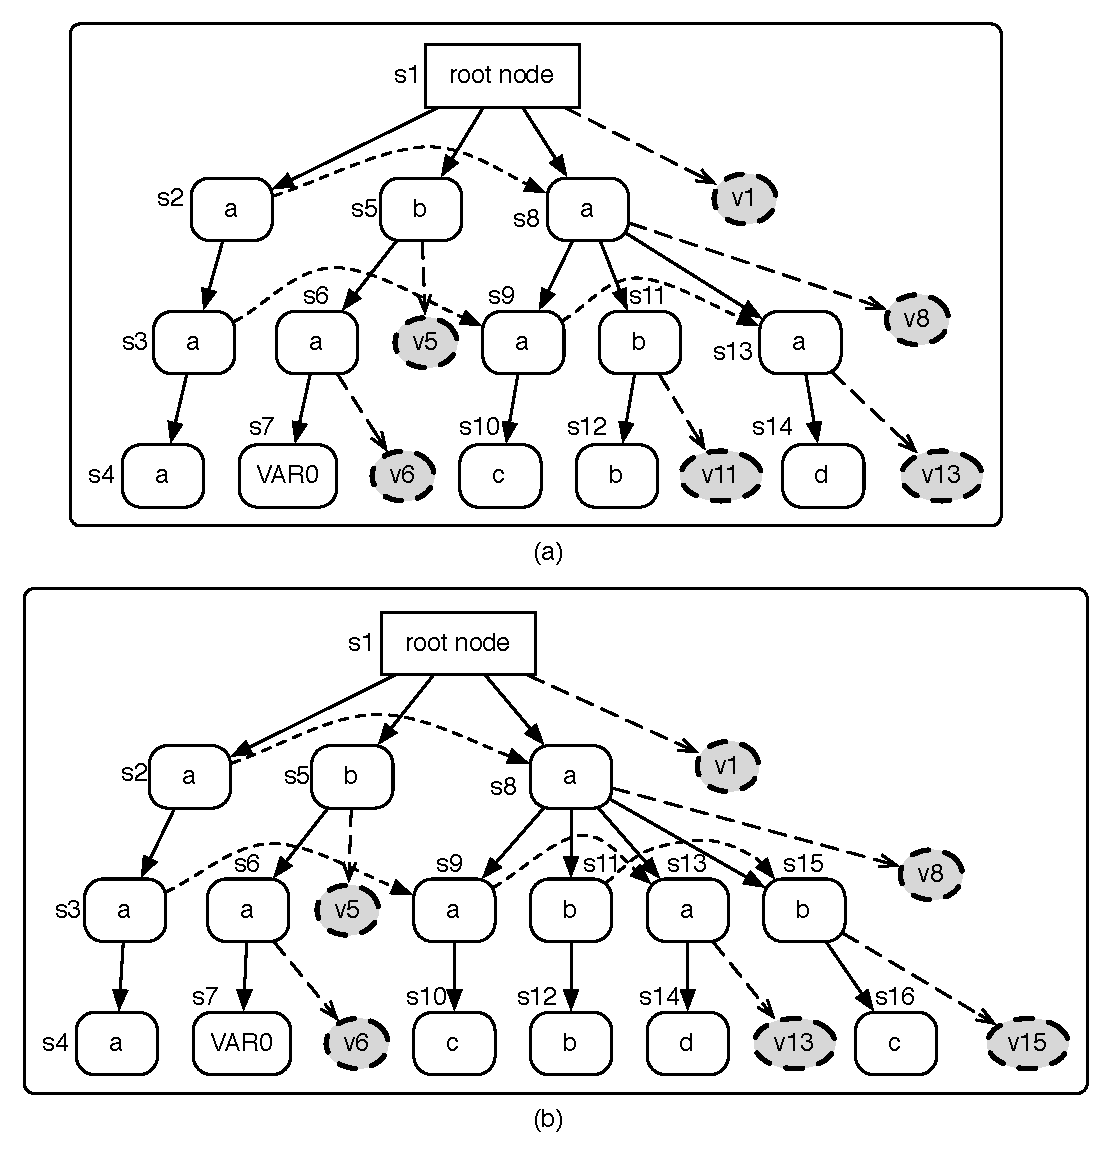
\includegraphics[scale=0.6]{dtsa.pdf}
  \caption{DTSA before and after inserting answer \texttt{p(a,b,c)}.}
  \label{fig:dtsa_example}
\end{figure}
 
\subsubsection{Dynamic Threaded Sequential Automata}

The previously described mechanisms only work if we have the complete set of answers for the subsuming subgoal.
A new mechanism that deals with incomplete answer sets must be devised, so that after all current answers
are retrieved, the continuation stack can be used to retrieve newly inserted answers.

The Dynamic Threaded Sequential Automata extends the TSA with special transitions in states
were new transitions can be inserted or in states were no equivalence links exist.
Figure \ref{fig:dtsa_example} illustrates two DTSAs: (a) shows the converted TSA from Figure \ref{fig:tsa_example}, and
(b) the resulting DTSA after inserting the answer \texttt{p(a,b,c)}.

During answer retrieval, if no answer is found and the top of the continuation stack contains
a transition to a special state, the process stops and the continuation stack is saved along the last state
visited.
Later on, when new answers must be retrieved, the last state is used to transform the stack to account for new states that
were introduced during the insertion of new terms. If the new stack contains a valid transition, it
can now be used as usual.

For example, retrieving answers to subgoal \texttt{p(a,X,c)} from the DTSA (a) in Figure
\ref{fig:dtsa_example} results in the answer \texttt{p(a,a,c)} and a continuation formed by the last
visited state $s13$ and the stack containing (from bottom to top): $[s1 \rightarrow v1, s8 \rightarrow v8, s13 \rightarrow v13]$.
After the new answer \texttt{p(a,b,c)} is inserted into the DTSA in Figure \ref{fig:dtsa_example} and
a consumer is resumed to consume new answers, it checks if new answers are available and the continuation stack
is thus transformed by using the last visited state $s13$ into: $[s1 \rightarrow v1, s8 \rightarrow s15]$. Now
the answer \texttt{p(a,b,c)} can be easily retrieved using the transition $s8 \rightarrow s15$.

\subsubsection{Table Space}

This new DTSA mechanism was implemented in XSB by extending the variant engine \cite{Rao-96}.

First, each subgoal frame for generator nodes now contains both an answer trie and a DTSA.
Answer tries are used to check for duplicate answers and the DTSA is created lazily, when a new subsumed node
first appears.

Each subsumed subgoal in the call trie keeps an answer return list that is built using the DTSA technique.
This answer list is used when variant goals of the subsumed goal are called, thus instead of using
the DTSA, answers are retrieved directly by traversing the linked list.

When a subgoal is marked as complete, the DTSA is deleted and the answer trie is converted into WAM instructions, a feature called
\textit{compiled trie code}. Answers for subsumed goals are then retrieved by using trie instructions
through the usual WAM backtracking mechanism.

\subsection{Time Stamped Tries} \label{sec:time_stamped_tries}

\textit{Time Stamped Tries} (TST) is another mechanism that was implemented in XSB
to support tabling by call subsumption \cite{Johnson-99}.

TST is a relatively simple technique based around the idea of augmenting a trie with information about the relative time
its terms were inserted. The time of insertion of each term is called its time stamp and is represented by a
positive integer. The time stamps are then used for incremental answer retrieval.

\begin{figure}[ht]
  \centering
    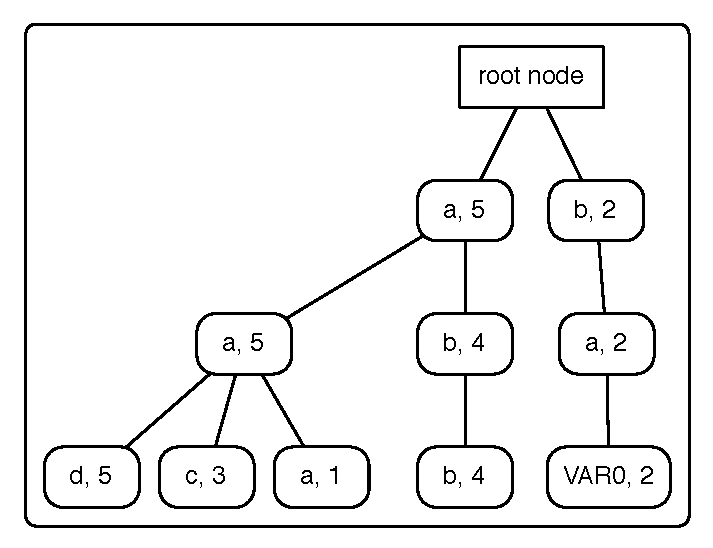
\includegraphics[scale=0.6]{tst_1.pdf}
  \caption{Time Stamped Trie for subgoal \texttt{p(X,Y,Z)}.}
  \label{fig:tst_1}
\end{figure}

For each node in a trie, we extend it by including a time stamp. Along the augmented trie, the maximum time stamp
$T$ is also stored, thus allowing the insert mechanism to know the next time stamp to use for new trie paths.
An example TST for the subgoal \texttt{p(X,Y,Z)} is represented in Figure \ref{fig:tst_1}.
By looking at the leaf nodes, the order of answer insertion
can be readily known: \texttt{p(a,a,a)}, \texttt{p(b,a,VAR0)}, \texttt{p(a,a,c)}, \texttt{p(a,b,b)} and then
\texttt{p(a,a,d)}.

\subsubsection{New Answers}

The process of inserting a new answer into a TST starts by traversing matching nodes as long the stored symbols
match the new answer. If the current symbol does not match, the process changes from search to insert mode and
new nodes are inserted to represent a new trie path. Once the leaf node is created, each node from leaf to root
is traversed and its time stamp is updated to $T + 1$.

\begin{figure}[ht]
  \centering
    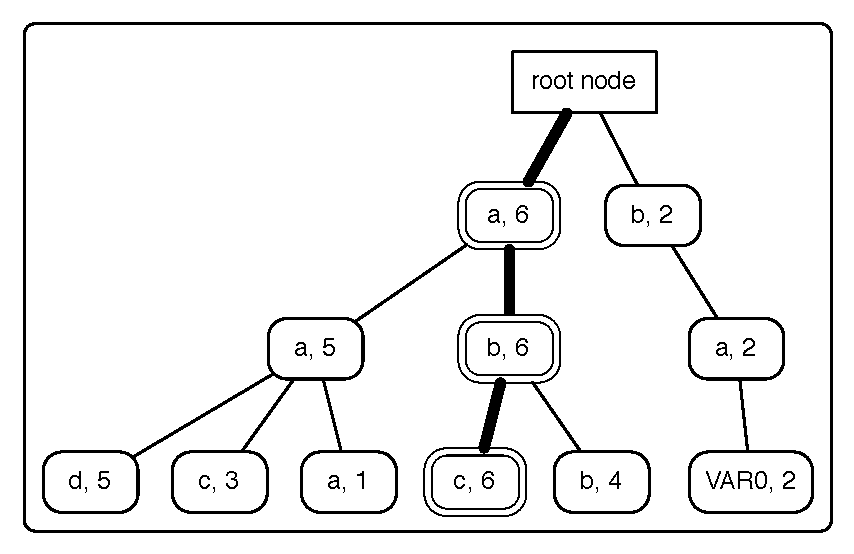
\includegraphics[scale=0.6]{tst_2.pdf}
  \caption{Time Stamped Trie from Figure \ref{fig:tst_1} after inserting the answer \texttt{p(a,b,c)}.}
  \label{fig:tst_2}
\end{figure}

Figure \ref{fig:tst_2} shows the TST from Figure \ref{fig:tst_1} after a new answer \texttt{p(a,b,c)} was inserted.
Note that each node from the answer leaf node to root node was updated with the new timestamp (6). Apart from
the time stamps, search and insertion in TSTs work exactly the same as tries.

\subsubsection{Retrieving Answers}

Retrieving all answers that are specific to a subsumed subgoal $G$ from a TST with answers from subgoal $G'$
works by navigating the TST and unifying the variable values that are assigned from $G'$ to $G$.
If we wanted to retrieve answers to the subgoal \texttt{p(a,a,X)} from the TST in Figure \ref{fig:tst_2},
during the subgoal call we determine the assignments relatively to \texttt{path(X,Y,Z)}: \texttt{X = a, Y = a, Z = VAR0},
and store them under the choice point. Then, these values $[a, a, VAR0]$ are then unified
with the trie symbols, thus finding answers that are specific to $G$.

Like tries, TSTs only store substitutions for variables, thus we must unify
the first sub-term $a$, then $a$ again and then the variable, which unifies with any symbol.
During the unification process, if a variable appears multiple times, it must unify with
any previous sub-term assignment.

Time stamps guide the answer unification process by filtering transitions to already explored branches, where
answers were already retrieved, thus avoiding repeated answers.

The unification process that finds new answers by using a time stamp is separated from the process
of unifying the retrieved answers with the subsumed subgoal. This \textit{two-tier mechanism} is key to the space and time
efficiency of the design of TSTs \cite{Johnson-99} and allows identification of all relevant answers that have
been added since the last time a search operation was done by using the time stamp.

\subsubsection{Table Space}

The table space in this technique extends the variant table space by
using TSTs instead of answer tries for subsuming goals.
 
Each subsumed subgoal in a call trie stores the last search time stamp $t$. The process of
incrementally searching for new answers in a TST will use $t$ and update it after the process completes.
When a subsumptive subgoal is first called $t$ is set to $0$, thus initially allowing the retrieval of all
relevant answers.

The subgoal in the call trie also stores an answer return list. Each time new answers are identified, they are appended
to this linked list. The original subsumptive consumer and its variant subgoals will then consume answers from it. If no
new answers can be retrieved from the list, the TST process is employed to identify more answers from the subsuming TST,
inserting them into the list.

Each TST node maintains a time stamp index which stores all transitions in reverse order.
It is not until a subsumed subgoal is first called that all time stamp related structures are created, thus
allowing a more efficient use of space.

Like DTSAs, the TST indexing mechanism is only used in incomplete subsuming calls, for complete calls
the more specific goals all use compiled trie instructions, and unification is performed naturally at
the WAM engine level.

The biggest advantage of using TSTs instead of DTSAs is in terms of space complexity. In TSTs, the maximum table space
used is at most twice that of the variant engine, because each node must contain both the time stamp and the time stamp index.
For DTSAs, the space used is at least double, but in the worst
case can be quadratic. DTSA is at advantage in terms of speed, because it supports identification of answers and
unification in one step, thus answers can share some elementary unifications. In TSTs, identifying answers
and doing answer unification is a two step process, thus it takes more time to construct all answers. 

\subsection{Finding subsuming goals}

Both DTSA and TST use a similar method that given a call trie $C$ and a subgoal $G$
is able to find a subgoal $G'$ that subsumes $G$.

The search is performed by recursively backtracking through the call trie $C$, trying
to match the node symbols with sub-terms or symbols from $G$.

A non-variable symbol from $G$ must only match with an identical symbol from $C$ and
these types of unifications are always tried first.
If the current trie symbol is a variable, for example \texttt{X}, on the first occurrence \texttt{X}
is bound to the respective $G$ sub-term
and match succeeds; on the next occurrences of \texttt{X}, the current sub-term from $G$ must
be identical to the term bound to \texttt{X}. Through the backtracking process, bound variables are
always tried before unbound variables.

Favoring constant values before variables, results in a mechanism that finds \textit{minimally subsuming calls}.
Also, if there is some variant call $G''$ in $C$, $G''$ is found before any other subgoal. If no variant 
or no subsuming call are found, it is possible to save the trie node to insert a new variant call.
This trie node is where the first backtracking occurred or when the first occurrence of
an already seen $G$ variable that could not be paired to a bound trie variable, and instead
must be bound to an unbound trie variable for the process to continue.
The new variant path is then used to keep information about the subsumed goal state in
the leaf call trie node.

\begin{figure}[ht]
  \centering
    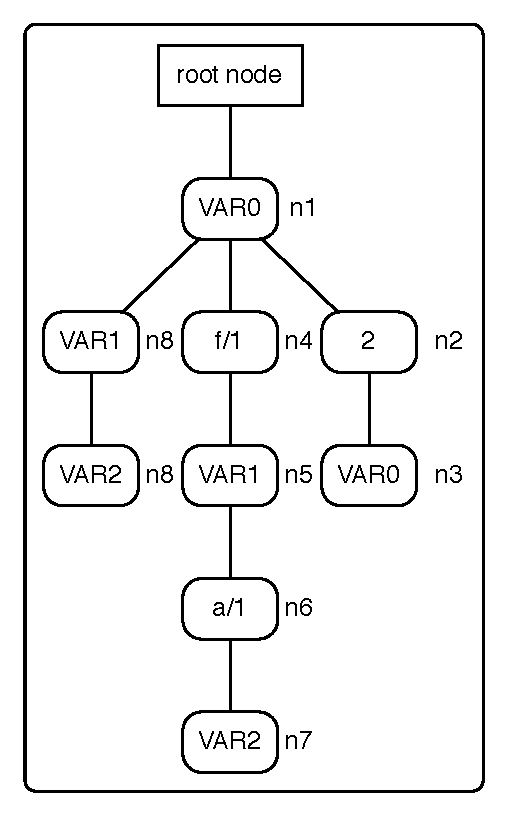
\includegraphics[scale=0.6]{sub_call_search.pdf}
  \caption{Call trie for predicate \texttt{p/3}.}
  \label{fig:sub_call_search}
\end{figure}

For illustration purposes, the Figure \ref{fig:sub_call_search} represents a call trie for the predicate \texttt{p/3}.
The first subgoal called was \texttt{p(X,2,X)}, followed by \texttt{p(X,f(Y),a(Z))} and finally \texttt{p(X,Y,Z)}.

If the subgoal \texttt{p(X,2,X)} is called once again, the algorithm described above
should find the variant subgoal represented by the leaf node $n3$. First, we unify the trie variable
\texttt{VAR0} with \texttt{X} (node $n1$), hence we must also mark the \texttt{X} variable as \textit{seen},
because if the same variable appears again it must unify with the same trie variable for a variant path
to exist. Next, \texttt{2} easily unifies with trie node $n2$ and unification proceeds. In trie node $n3$,
the current call term is \texttt{X} and we also have a variable in the trie node. As \texttt{X} was already seen before,
it must unify with \textit{VAR0} again, it does and a variant path is found. Please note that if
the trie symbol at node $n3$ was \texttt{VAR1}, the process could proceed but a variant path would be impossible
to exist, and a subsuming subgoal would be found, as \texttt{p(VAR0,2,VAR1)} subsumes \texttt{path(VAR0,2,VAR0)}.
In this case, a variant path could created by resuming the trie insert operation at node $n2$ to insert
a \texttt{VAR0} node.

For a more complex example, the subgoal \texttt{p(2,f(X),a(2))} is now called for the same call trie. First,
the algorithm tries to find a trie node with the symbol \texttt{2}, it does not and a variant path
can not be possibly found in this call trie. Next, the algorithm tries to unify with bound variables, but as the process
has just started, only unbound variables can be found and \texttt{VAR0} is unified with \texttt{2} (node $n1$).
The functor term \texttt{f/1} is the next symbol on the subgoal and the first trie node that must be tried is $n4$,
because it contains a non-variable symbol. The next term is \texttt{X} and it can unify with \texttt{VAR1} (node $n5$).
Next, the term symbol \texttt{a/1} matches with trie node $n6$ and the process proceeds. Note that if we failed
at this point, the process would backtrack to node $n2$ and node $n8$ would be tried next, which would
lead to a more general subgoal. Back to node $n6$, the last term symbol \texttt{2} can match with node $n7$, as it is the only trie
node available and it is an unbound variable. If the variable was bound, like \texttt{VAR0} for instance,
the process would check if the current term symbol unifies with the variable binding made before (\texttt{VAR0 = 2}) and
it would also succeed. As node $n7$ is a leaf node, the process finishes and a subsumptive path is found.
The following variable bindings were made: \texttt{VAR0 = 2}, \texttt{VAR1 = X}, and \texttt{VAR2 = 2}.
